\section{word clouds}\label{sec:wordclouds}

This section presents the word clouds generated as part of the exploratory data analysis.
Figure \ref{fig:wordcloud-all} shows the word cloud for all the documents in the data set. 
Figures \ref{fig:wordcloud-ISTJ} to \ref{fig:wordcloud-ENTJ} show the word clouds generated from documents when partitioned according to the Myers-Briggs type label of the documents.
The word cloud for each partitioned data set clearly shows the MBTI label partitioning the data set to also be a common word in that partition of documents.

\begin{figure}[htp] 
  \caption{word cloud generated from all the documents in the data set. Visualises the most common words in the whole data set.}
  \label{fig:wordcloud-all}
  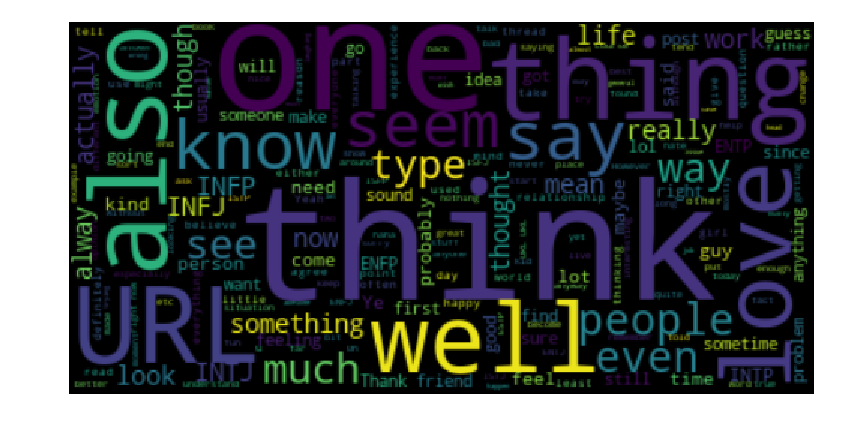
\includegraphics[scale=0.65]{wordclouds/wordcloud_all.pdf}
\end{figure}

\begin{figure}[htp] 
  \caption{word cloud generated from all documents with the ISTJ Myers-Briggs type indicator. As we can see, "ISTJ" is a common word for this subset of documents.}
  \label{fig:wordcloud-ISTJ}
  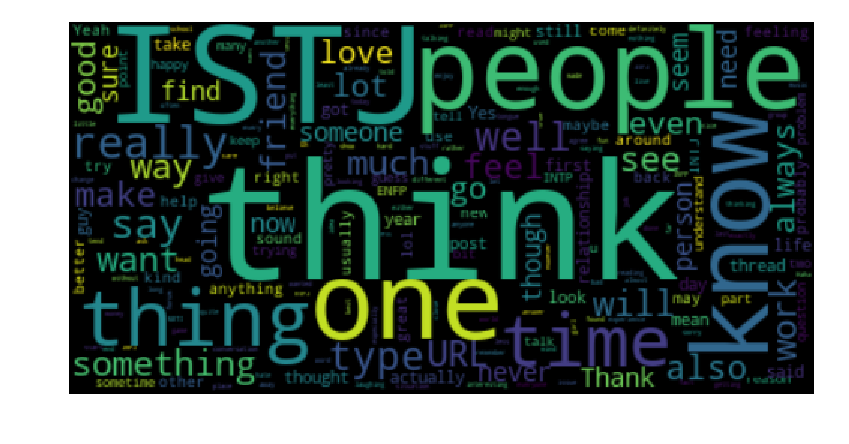
\includegraphics[scale=0.65]{wordclouds/wordcloud_ISTJ.pdf}
\end{figure}

\begin{figure}[htp] 
  \caption{word cloud generated from all documents with the ISFJ Myers-Briggs type indicator. As we can see, "ISFJ" is a common word for this subset of documents.}
  \label{fig:wordcloud-ISFJ}
  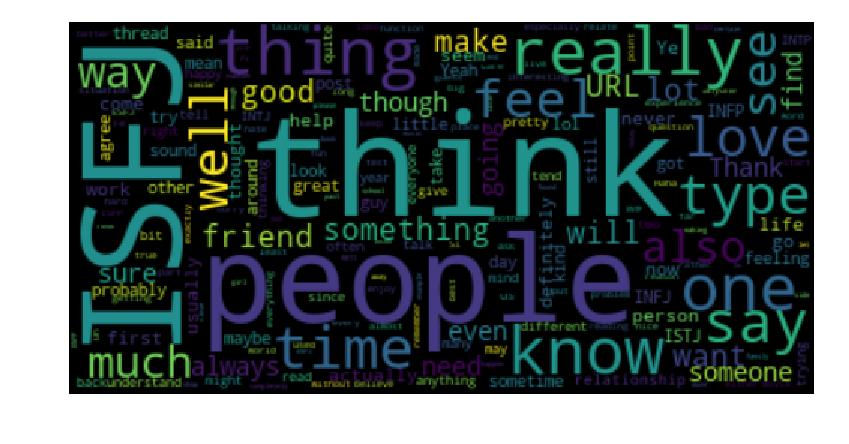
\includegraphics[scale=0.65]{wordclouds/wordcloud_ISFJ.pdf}
\end{figure}

\begin{figure}[htp] 
  \caption{word cloud generated from all documents with the INFJ Myers-Briggs type indicator. As we can see, "INFJ" is a common word for this subset of documents.}
  \label{fig:wordcloud-INFJ}
  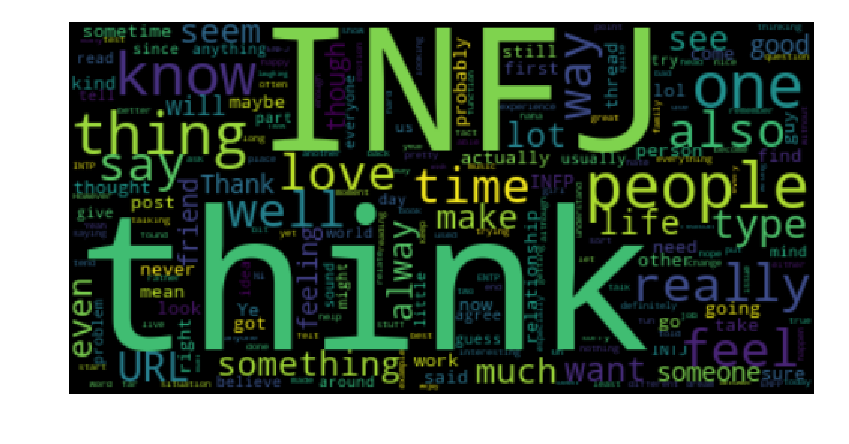
\includegraphics[scale=0.65]{wordclouds/wordcloud_INFJ.pdf}
\end{figure}

\begin{figure}[htp] 
  \caption{word cloud generated from all documents with the INTJ Myers-Briggs type indicator. As we can see, "INTJ" is a common word for this subset of documents.}
  \label{fig:wordcloud-INTJ}
  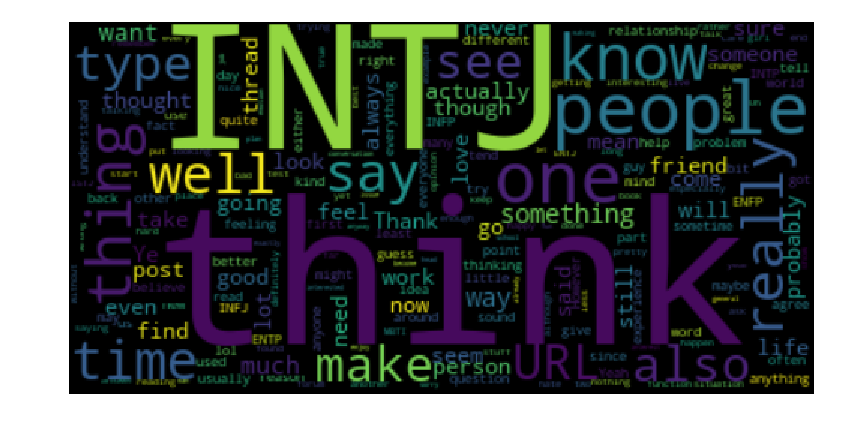
\includegraphics[scale=0.65]{wordclouds/wordcloud_INTJ.pdf}
\end{figure}

\begin{figure}[htp] 
  \caption{word cloud generated from all documents with the ISTP Myers-Briggs type indicator. As we can see, "ISTP" is a common word for this subset of documents.}
  \label{fig:wordcloud-ISTP}
  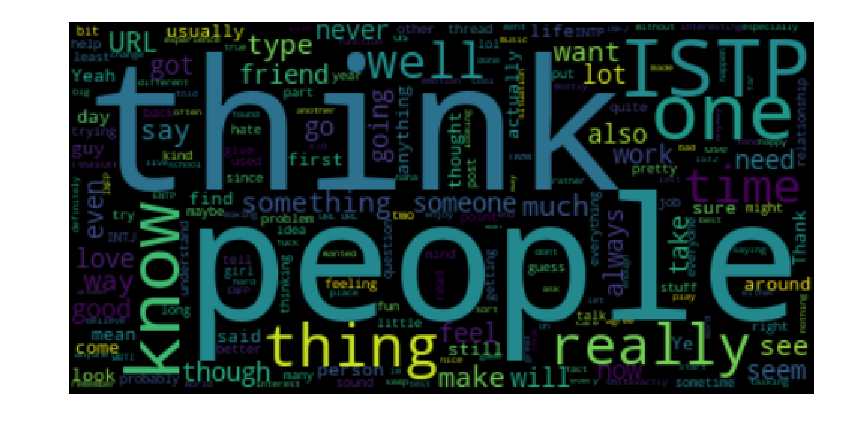
\includegraphics[scale=0.65]{wordclouds/wordcloud_ISTP.pdf}
\end{figure}

\begin{figure}[htp] 
  \caption{word cloud generated from all documents with the ISFP Myers-Briggs type indicator. As we can see, "ISFP" is a common word for this subset of documents.}
  \label{fig:wordcloud-ISFP}
  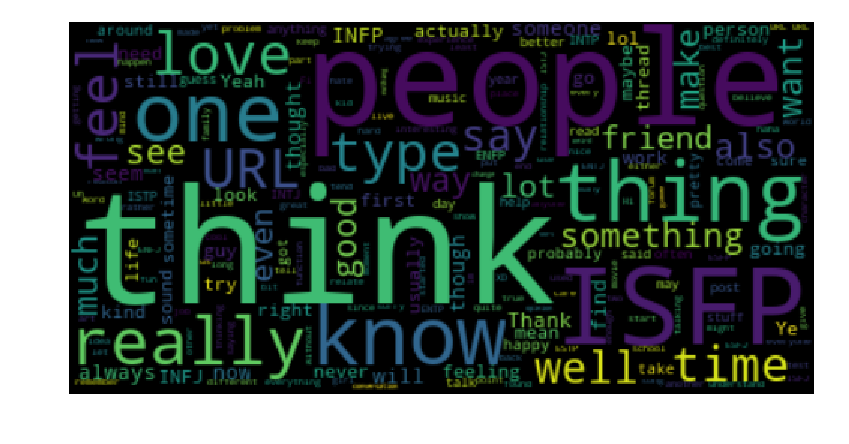
\includegraphics[scale=0.65]{wordclouds/wordcloud_ISFP.pdf}
\end{figure}

\begin{figure}[htp] 
  \caption{word cloud generated from all documents with the INFP Myers-Briggs type indicator. As we can see, "INFP" is a common word for this subset of documents.}
  \label{fig:wordcloud-INFP}
  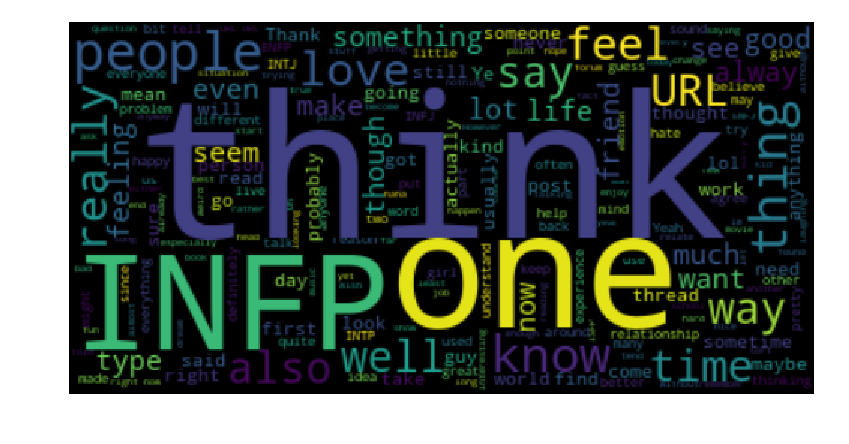
\includegraphics[scale=0.65]{wordclouds/wordcloud_INFP.pdf}
\end{figure}

\begin{figure}[htp] 
  \caption{word cloud generated from all documents with the INTP Myers-Briggs type indicator. As we can see, "INTP" is a common word for this subset of documents.}
  \label{fig:wordcloud-INTP}
  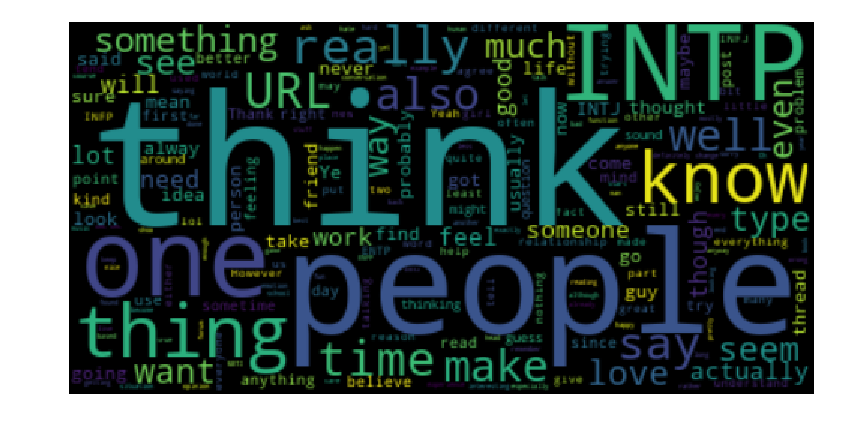
\includegraphics[scale=0.65]{wordclouds/wordcloud_INTP.pdf}
\end{figure}

\begin{figure}[htp] 
  \caption{word cloud generated from all documents with the ESTP Myers-Briggs type indicator. As we can see, "ESTP" is a common word for this subset of documents.}
  \label{fig:wordcloud-ESTP}
  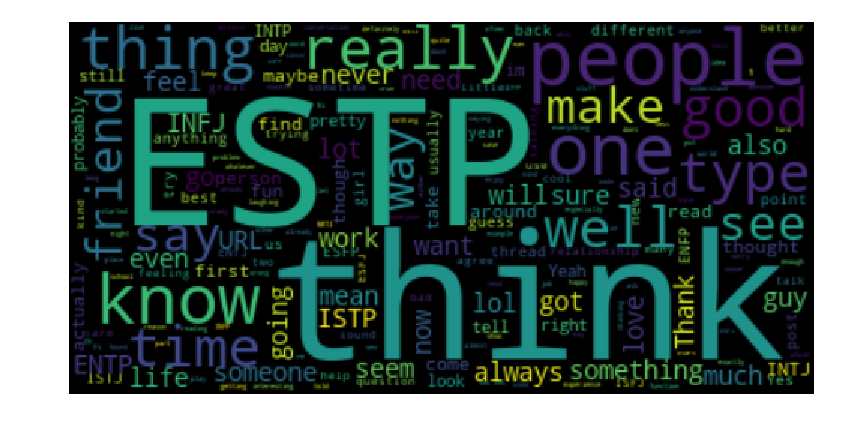
\includegraphics[scale=0.65]{wordclouds/wordcloud_ESTP.pdf}
\end{figure}

\begin{figure}[htp] 
  \caption{word cloud generated from all documents with the ESFP Myers-Briggs type indicator. As we can see, "ESFP" is a common word for this subset of documents.}
  \label{fig:wordcloud-ESFP}
  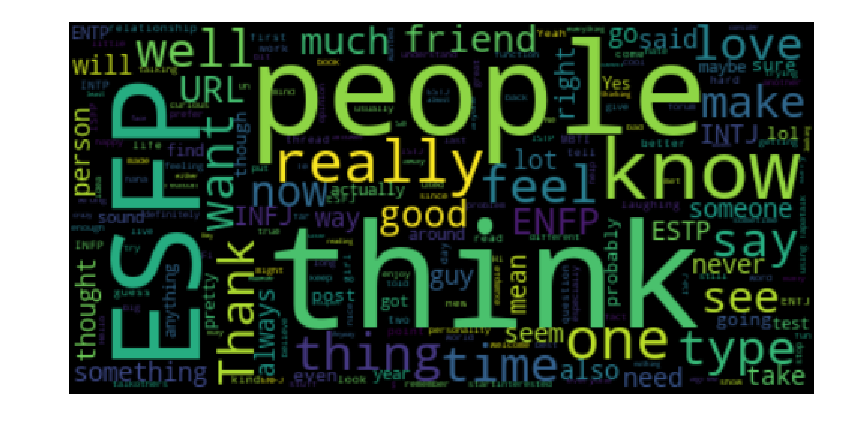
\includegraphics[scale=0.65]{wordclouds/wordcloud_ESFP.pdf}
\end{figure}

\begin{figure}[htp] 
  \caption{word cloud generated from all documents with the ENFP Myers-Briggs type indicator. As we can see, "ENFP" is a common word for this subset of documents.}
  \label{fig:wordcloud-ENFP}
  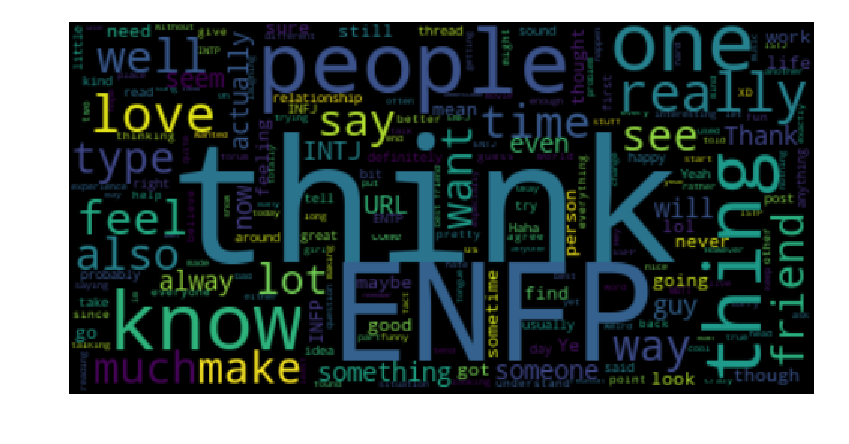
\includegraphics[scale=0.65]{wordclouds/wordcloud_ENFP.pdf}
\end{figure}

\begin{figure}[htp] 
  \caption{word cloud generated from all documents with the ENTP Myers-Briggs type indicator. As we can see, "ENTP" is a common word for this subset of documents.}
  \label{fig:wordcloud-ENTP}
  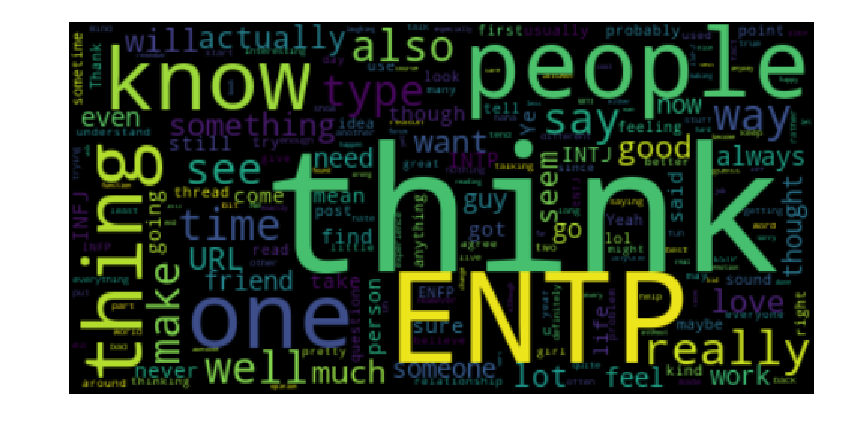
\includegraphics[scale=0.65]{wordclouds/wordcloud_ENTP.pdf}
\end{figure}

\begin{figure}[htp] 
  \caption{word cloud generated from all documents with the ESTJ Myers-Briggs type indicator. As we can see, "ESTJ" is a common word for this subset of documents.}
  \label{fig:wordcloud-ESTJ}
  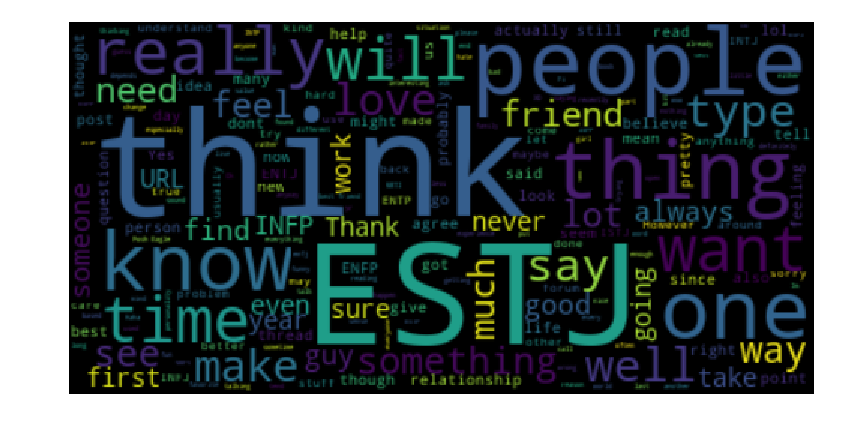
\includegraphics[scale=0.65]{wordclouds/wordcloud_ESTJ.pdf}
\end{figure}

\begin{figure}[htp] 
  \caption{word cloud generated from all documents with the ESFJ Myers-Briggs type indicator. As we can see, "ESFJ" is a common word for this subset of documents.}
  \label{fig:wordcloud-ESFJ}
  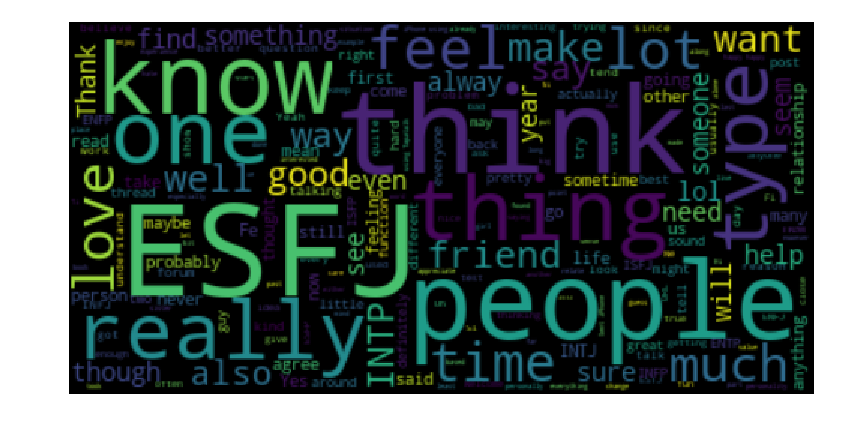
\includegraphics[scale=0.65]{wordclouds/wordcloud_ESFJ.pdf}
\end{figure}

\begin{figure}[htp] 
  \caption{word cloud generated from all documents with the ENFJ Myers-Briggs type indicator. As we can see, "ENFJ" is a common word for this subset of documents.}
  \label{fig:wordcloud-ENFJ}
  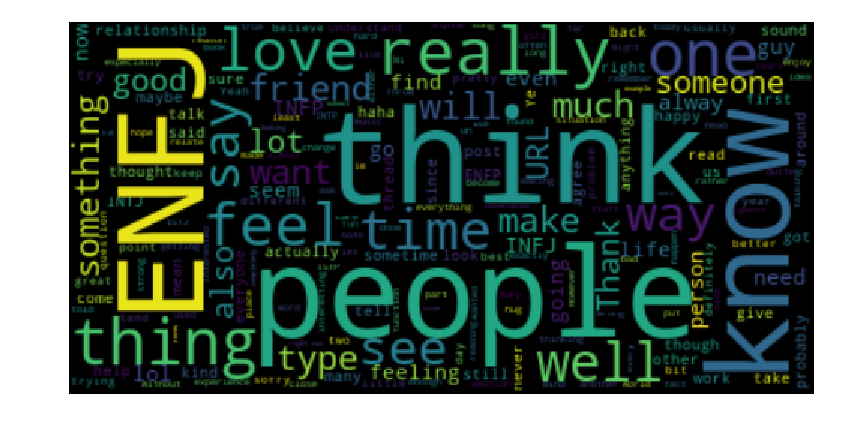
\includegraphics[scale=0.65]{wordclouds/wordcloud_ENFJ.pdf}
\end{figure}

\begin{figure}[htp] 
  \caption{word cloud generated from all documents with the ENTJ Myers-Briggs type indicator. As we can see, "ENTJ" is a common word for this subset of documents.}
  \label{fig:wordcloud-ENTJ}
  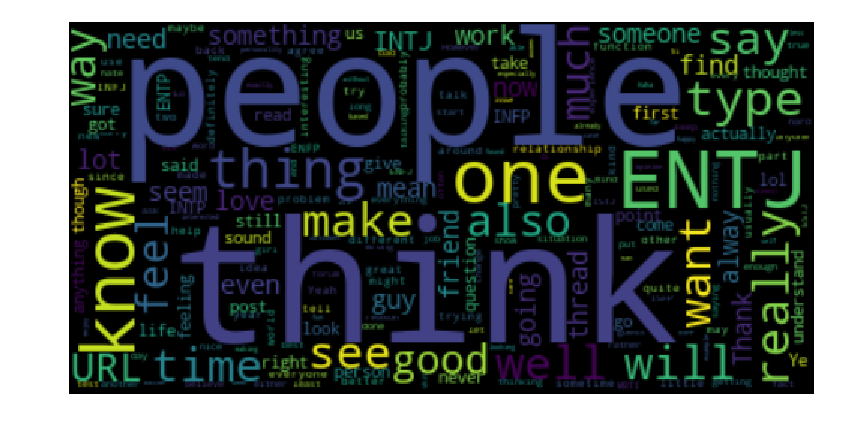
\includegraphics[scale=0.65]{wordclouds/wordcloud_ENTJ.pdf}
\end{figure}